%%%%cls文件默认改用ctexart类,如果使用使用cctart类,请使用xelatex并修改SCIS2022cn.cls文件对应内容;
% !TEX encoding = UTF-8
% !TEX program = pdflatex
%-----------------------------------------------------------------------
% 中国科学: 信息科学 中文模板, 请用 TexLive 编译
% http://scis.scichina.com
%-----------------------------------------------------------------------

\documentclass{SCIS2022cn}
%%%%%%%%%%%%%%%%%%%%%%%%%%%%%%%%%%%%%%%%%%%%%%%%%%%%%%%
%%% 作者附加的定义
%%% 常用环境已经加载好, 不需要重复加载
%%%%%%%%%%%%%%%%%%%%%%%%%%%%%%%%%%%%%%%%%%%%%%%%%%%%%%%
\standardtilde \let\standardtilde=\relax
\usepackage{CJK}
\usepackage{graphicx}
\usepackage{float} 
\usepackage{subfigure}
\usepackage{listings}
\usepackage{xcolor}


%%%%%%%%%%%%%%%%%%%%%%%%%%%%%%%%%%%%%%%%%%%%%%%%%%%%%%%
%%% 图片格式
\renewcommand{\figurename}{图}
\renewcommand{\captionlabeldelim}{.~}
\renewcommand{\thesubfigure}{(\roman{subfigure})}
\makeatletter \renewcommand{\@thesubfigure}{\thesubfigure \space}
\renewcommand{\p@subfigure}{} \makeatother
%%%%%%%%%%%%%%%%%%%%%%%%%%%%%%%%%%%%%%%%%%%%%%%%%%%%%%%

%%%%%%%%%%%%%%%%%%%%%%%%%%%%%%%%%%%%%%%%%%%%%%%%%%%%%%%
%%% 代码格式
\lstset{
columns=fixed,
numbers=left,                                        % 在左侧显示行号
numberstyle=\tiny\color{gray},                       % 设定行号格式
frame=none,                                          % 不显示背景边框
breaklines=true,                                     % 代码过长则换行
backgroundcolor=\color[RGB]{245,245,244},            % 设定背景颜色
keywordstyle=\color[RGB]{40,40,255},                 % 设定关键字颜色
numberstyle=\footnotesize\color{darkgray},           
commentstyle=\it\color[RGB]{0,96,96},                % 设置代码注释的格式
stringstyle=\rmfamily\slshape\color[RGB]{128,0,0},   % 设置字符串格式
showstringspaces=false,                              % 不显示字符串中的空格
}
%%%%%%%%%%%%%%%%%%%%%%%%%%%%%%%%%%%%%%%%%%%%%%%%%%%%%%%

%%%%%%%%%%%%%%%%%%%%%%%%%%%%%%%%%%%%%%%%%%%%%%%%%%%%%%%
%%% 开始
%%%%%%%%%%%%%%%%%%%%%%%%%%%%%%%%%%%%%%%%%%%%%%%%%%%%%%%
\begin{document}

%%%%%%%%%%%%%%%%%%%%%%%%%%%%%%%%%%%%%%%%%%%%%%%%%%%%%%%
%%% 作者不需要修改此处信息
\ArticleType{论文}
\Year{2022}
\BeginPage{1}
%%%%%%%%%%%%%%%%%%%%%%%%%%%%%%%%%%%%%%%%%%%%%%%%%%%%%%%

\title{Developing a Java Game from Scratch}{Developing a Java Game from Scratch}

\author[1]{王鹏}{Peng Wang}{{191220112@smail.nju.edu.cn}}

\address[1]{南京大学, 南京 210023}{NJU, NanJing {\rm 210023}, China}

\abstract{
本项目的开发目标是完成一个模拟地牢的多人对战小游戏,
本项目在开发过程中主要的设计方法是面向对象的设计,并
使用了多线程、线程锁的技术,在多人对战的同步过程中,
使用NIO Selector作为多个客户端的管理方式,在项目
管理上,主要使用maven进行自动化构建、测试、插件管理
等,并使用一些自动化工具进行测试覆盖度报告和类图的生成。
}

\keywords{开发目标,设计理念,技术问题,工程问题,课程感言}

\maketitle

\section{开发目标}

\subsection{游戏介绍}

本项目开发的是一个单人打怪(地牢探险)/多人对战(PVP)游戏,游戏设计灵感来源于
\href{http://www.chillyroom.com/zh/soul-knight/change-log}{《元气骑士》}。
在游戏的1.0版本,初步实现了单人打怪模式,怪物在看不到玩家的时候将随机游走,
在能够看到玩家(玩家接近且没有障碍物阻隔)时将在随机游走的同时向玩家发起攻击。
在2.0版本中实现了游戏状态、进度的保存与加载。在3.0版本,实现了多人联机对战,
不同玩家互相攻击,击败对方后可以得到对方的分数,最终击杀其他所有人的玩家获胜。

\subsection{玩法说明}

\subsubsection{1.0版本}

最初的版本,地图上会有墙体(不可击破、不可穿越)、石头(不可穿越、可以击破)、
树、草、花等场景实体,地图随机位置生成10个怪物。玩家通过WASD操纵自己的人物
(图\ref{Fig.sub.1})中的白色人物,Enter键攻击,经历重重困难,击败所有怪物
并到达终点(图\ref{Fig.sub.2})后获得胜利。

\begin{figure}[H]
    \centering
    \subfigure[游戏界面]{
    \label{Fig.sub.1}
    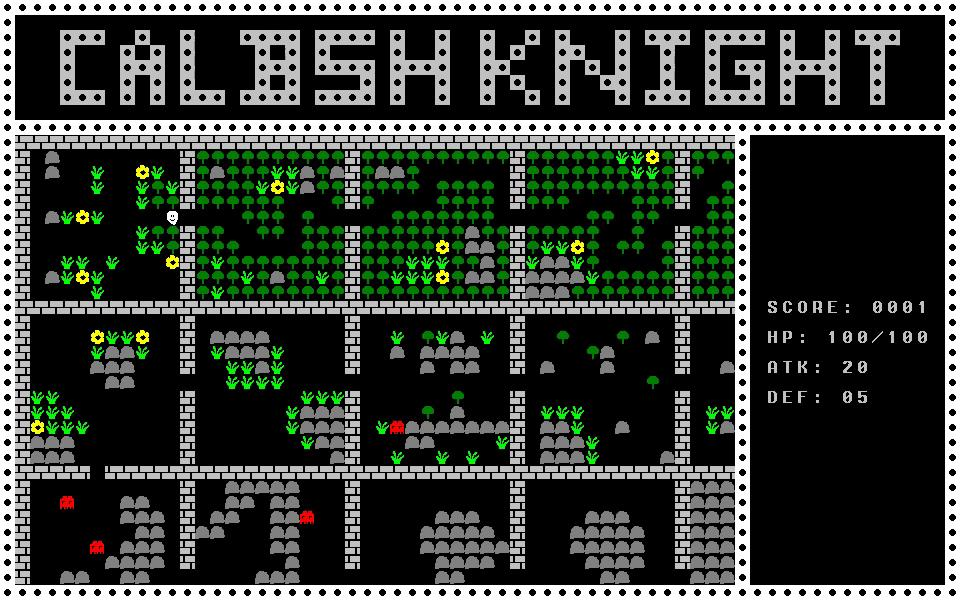
\includegraphics[width=0.30\textwidth]{ref/1-2-1-1.jpg}}
    \subfigure[到达终点]{
    \label{Fig.sub.2}
    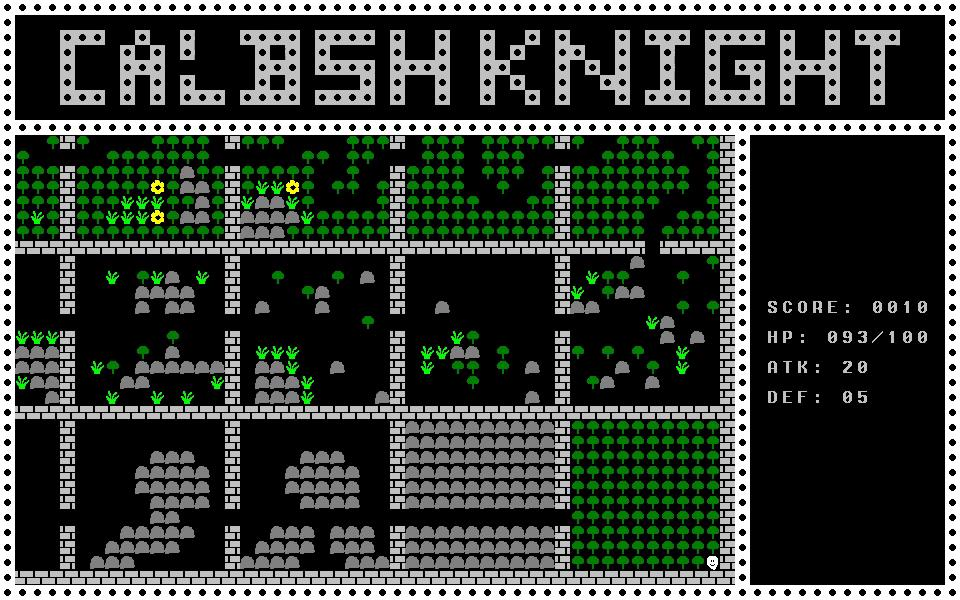
\includegraphics[width=0.30\textwidth]{ref/1-2-1-2.jpg}}
    \subfigure[游戏胜利]{
    \label{Fig.sub.3}
    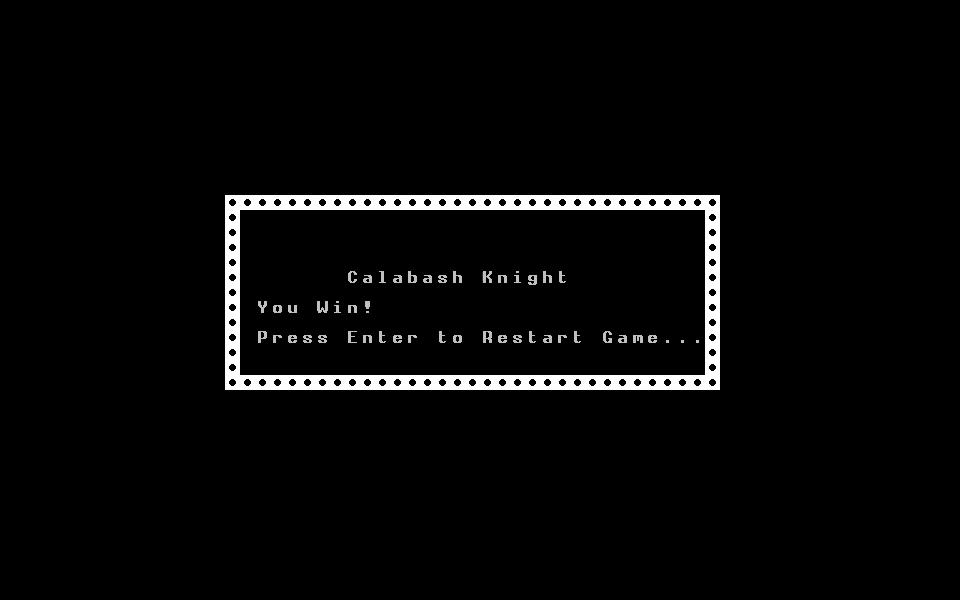
\includegraphics[width=0.30\textwidth]{ref/1-2-1-3.jpg}}
    \caption{1.0版本}
    \label{Fig.f121}
\end{figure}

\subsubsection{2.0版本}

在该版本中添加了地图编辑功能,游戏状态、过程存储与重载功能,玩家在游戏过程中
可以按下X键进行状态的存档,或按下R键进行游戏操作录制,在游戏的开始界面可以选
择LOAD RECORD进行加载。

\begin{figure}[H]
    \centering
    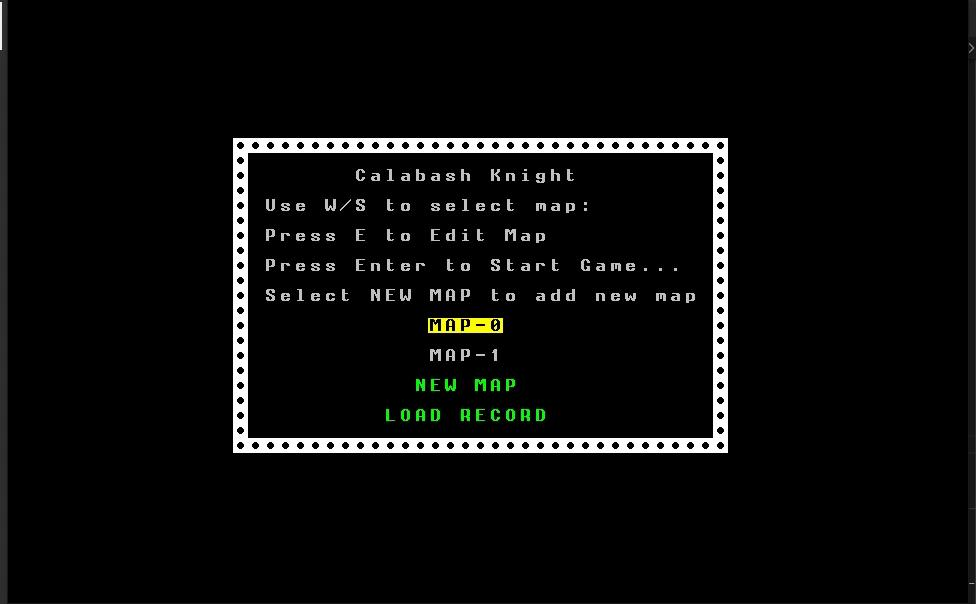
\includegraphics[width=0.7\textwidth]{ref/1-2-2-1.jpg}
    \caption{2.0版本开始界面}
    \label{Fig.f1221}
\end{figure}

在游戏开始前,可以在光标指向某个地图时按下E键编辑地图,或选中NEW MAP时按下Enter
键创建新地图,在创建新地图时,移动红色光标到目标位置,按下Enter键修改对应位置的
地图实体(灵感来源于经典坦克大战),如图\ref{Fig.f1222}。

\begin{figure}[H]
    \centering
    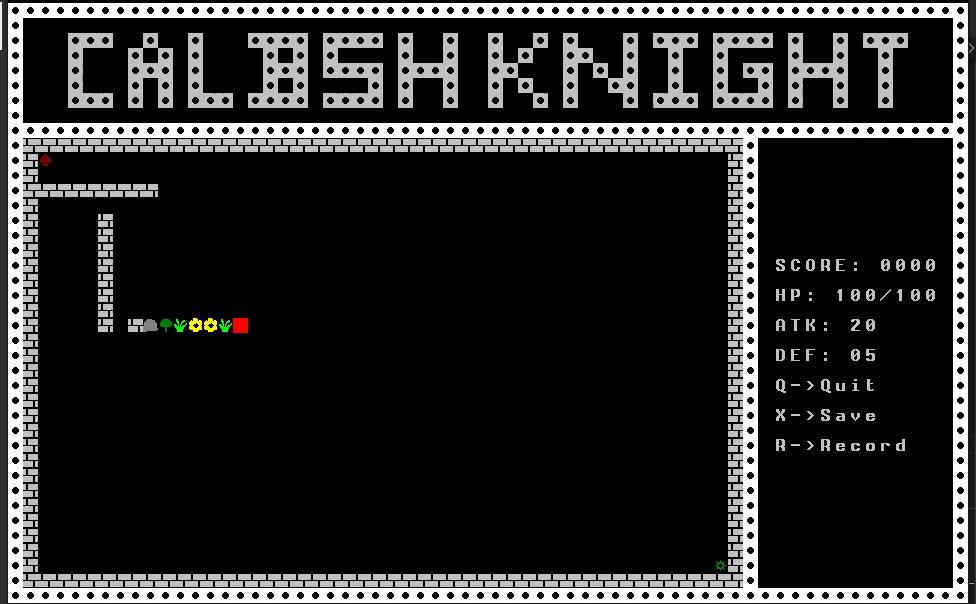
\includegraphics[width=0.7\textwidth]{ref/1-2-2-2.jpg}
    \caption{创建新地图}
    \label{Fig.f1222}
\end{figure}

在游戏过程中,按下X键记录状态,按下R键开始录制(图\ref{Fig.s1223}),再次按下R键
保存录制结果,重新进入游戏开始界面,选择LOAD RECORD可以加载保存的记录(图\ref{Fig.s1224}。
其中status开头的为记录的状态,record开头的为录制的操作(操作的第一条是状态)。载入
记录内容后不可继续操作角色,只能按N键播放记录中的操作(图\ref{Fig.s1225})直到记录播放结束。


\begin{figure}[H]
    \centering
    \subfigure[录制]{
    \label{Fig.s1223}
    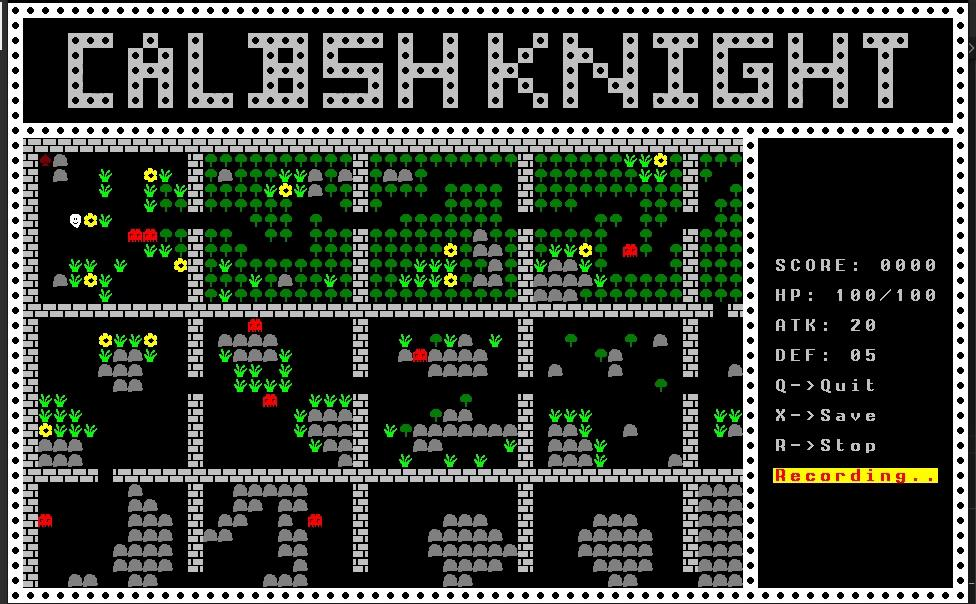
\includegraphics[width=0.30\textwidth]{ref/1-2-2-3.jpg}}
    \subfigure[加载]{
    \label{Fig.s1224}
    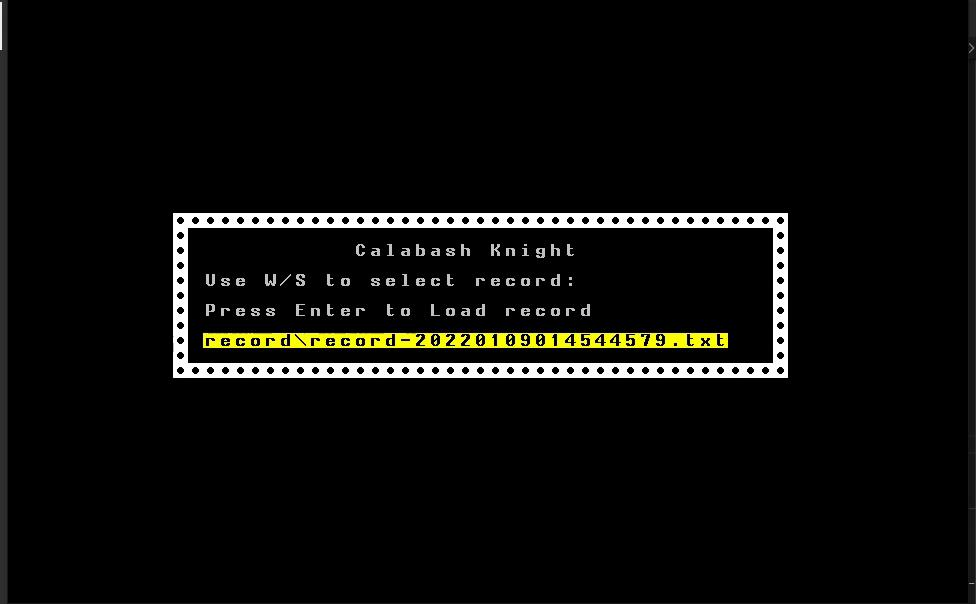
\includegraphics[width=0.30\textwidth]{ref/1-2-2-4.jpg}}
    \subfigure[播放]{
    \label{Fig.s1225}
    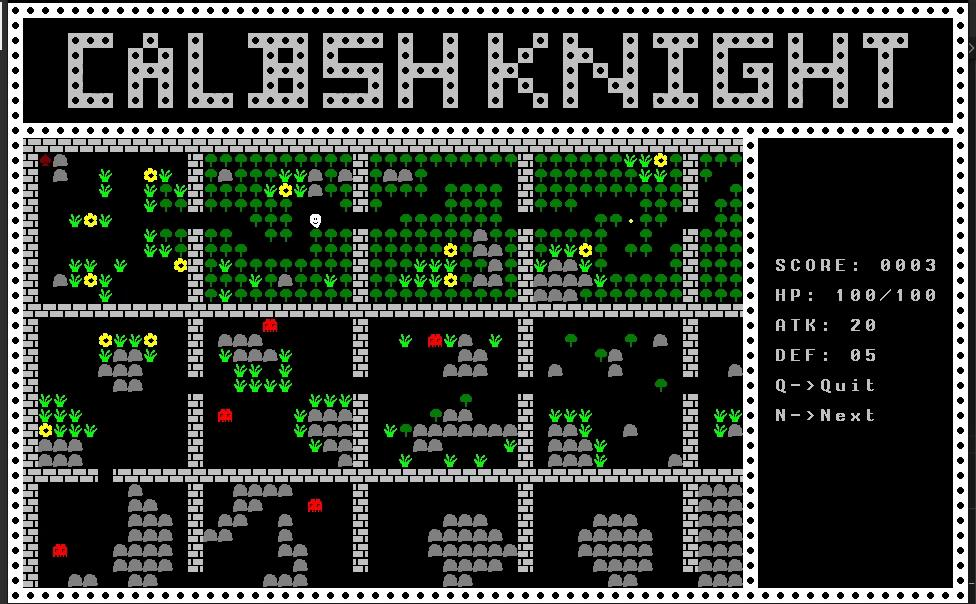
\includegraphics[width=0.30\textwidth]{ref/1-2-2-5.jpg}}
    \caption{录制与加载}
    \label{Fig.f122}
\end{figure}

\subsubsection{3.0版本}

该版本将单人打怪模式修改为多人对战模式(图\ref{Fig.s1231}),一位玩家启
动服务端(添加-s参数),其他玩家启动客户端(添加-c参数),形成联机网络
,玩家之间互相攻击,击败对方后可以获得对方的分数(图\ref{Fig.s1232}),
所有玩家初始分数为1,当得到与玩家数量相同的分数(击败其他所有玩家)
时获得游戏胜利(图\ref{Fig.s1233})。

\begin{figure}[H]
    \centering
    \subfigure[玩家对战]{
    \label{Fig.s1231}
    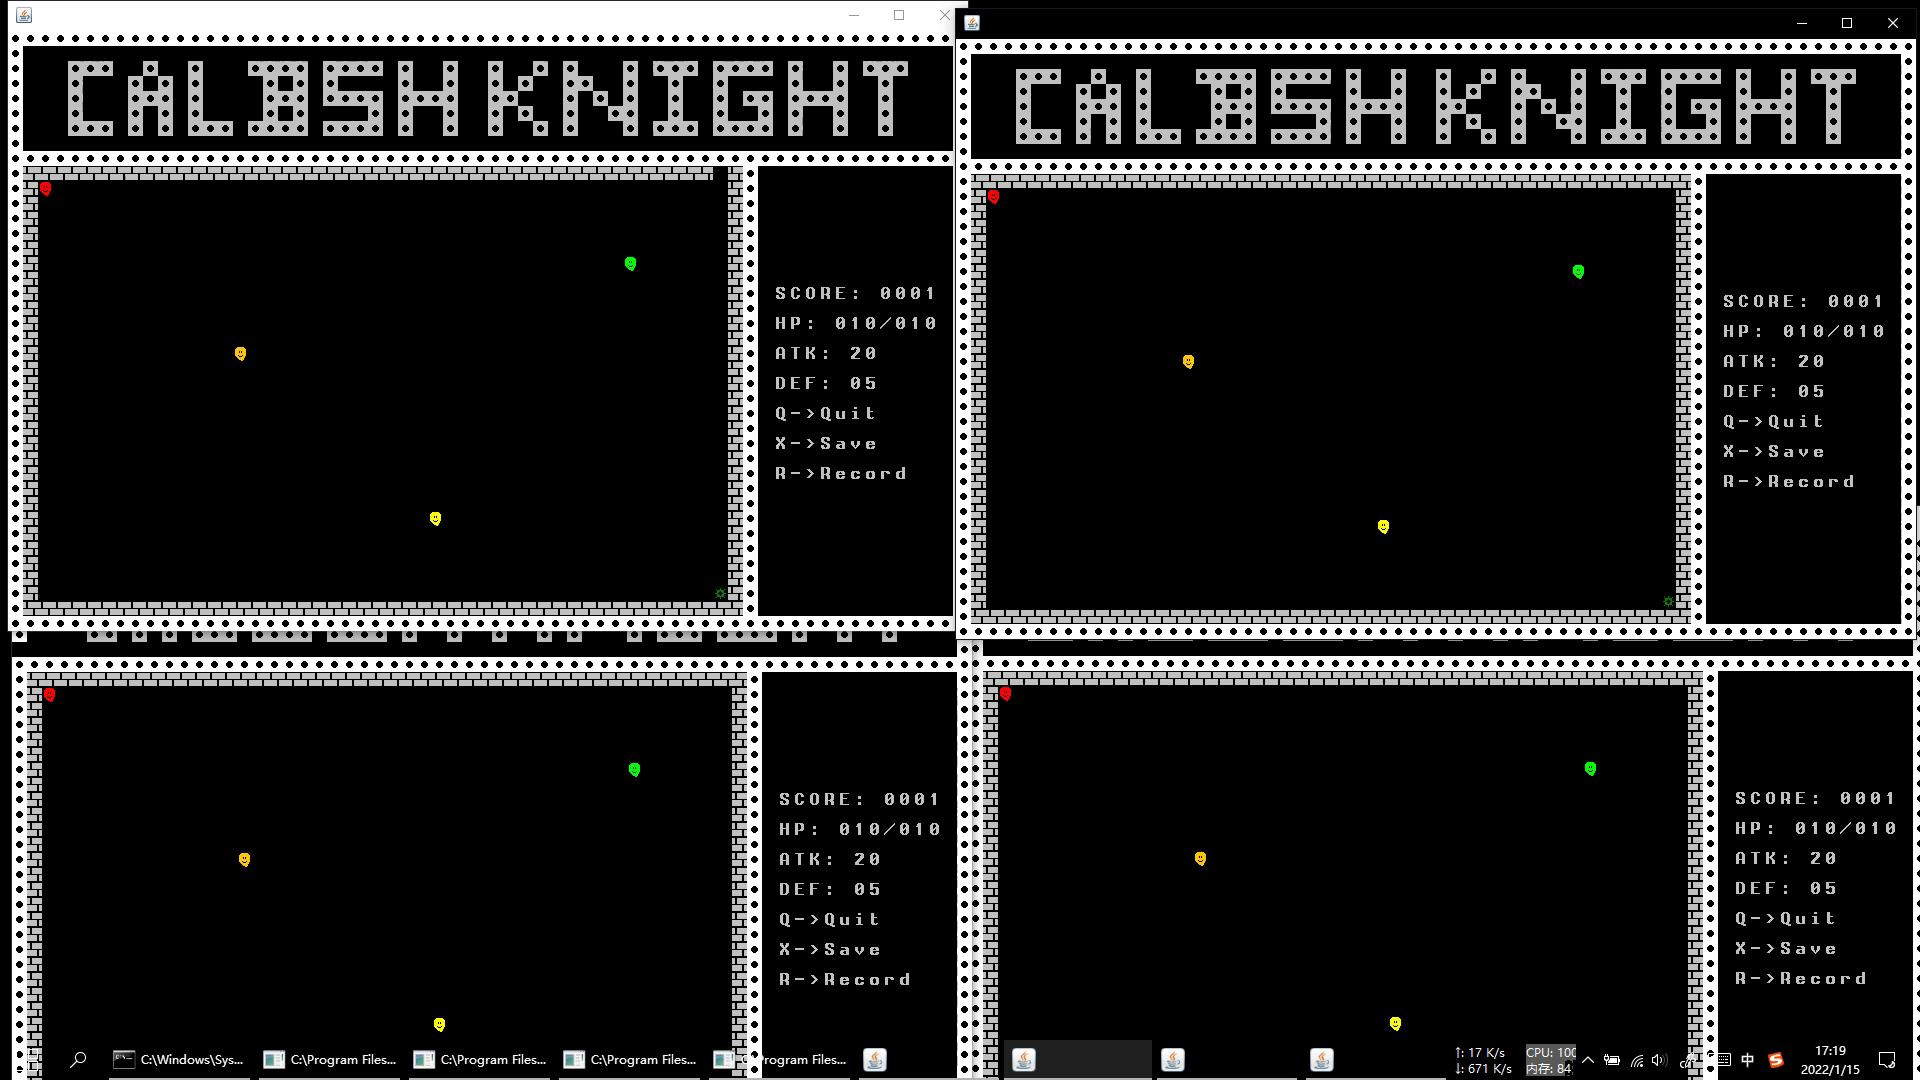
\includegraphics[width=0.30\textwidth]{ref/1-2-3-1.jpg}}
    \subfigure[击败]{
    \label{Fig.s1232}
    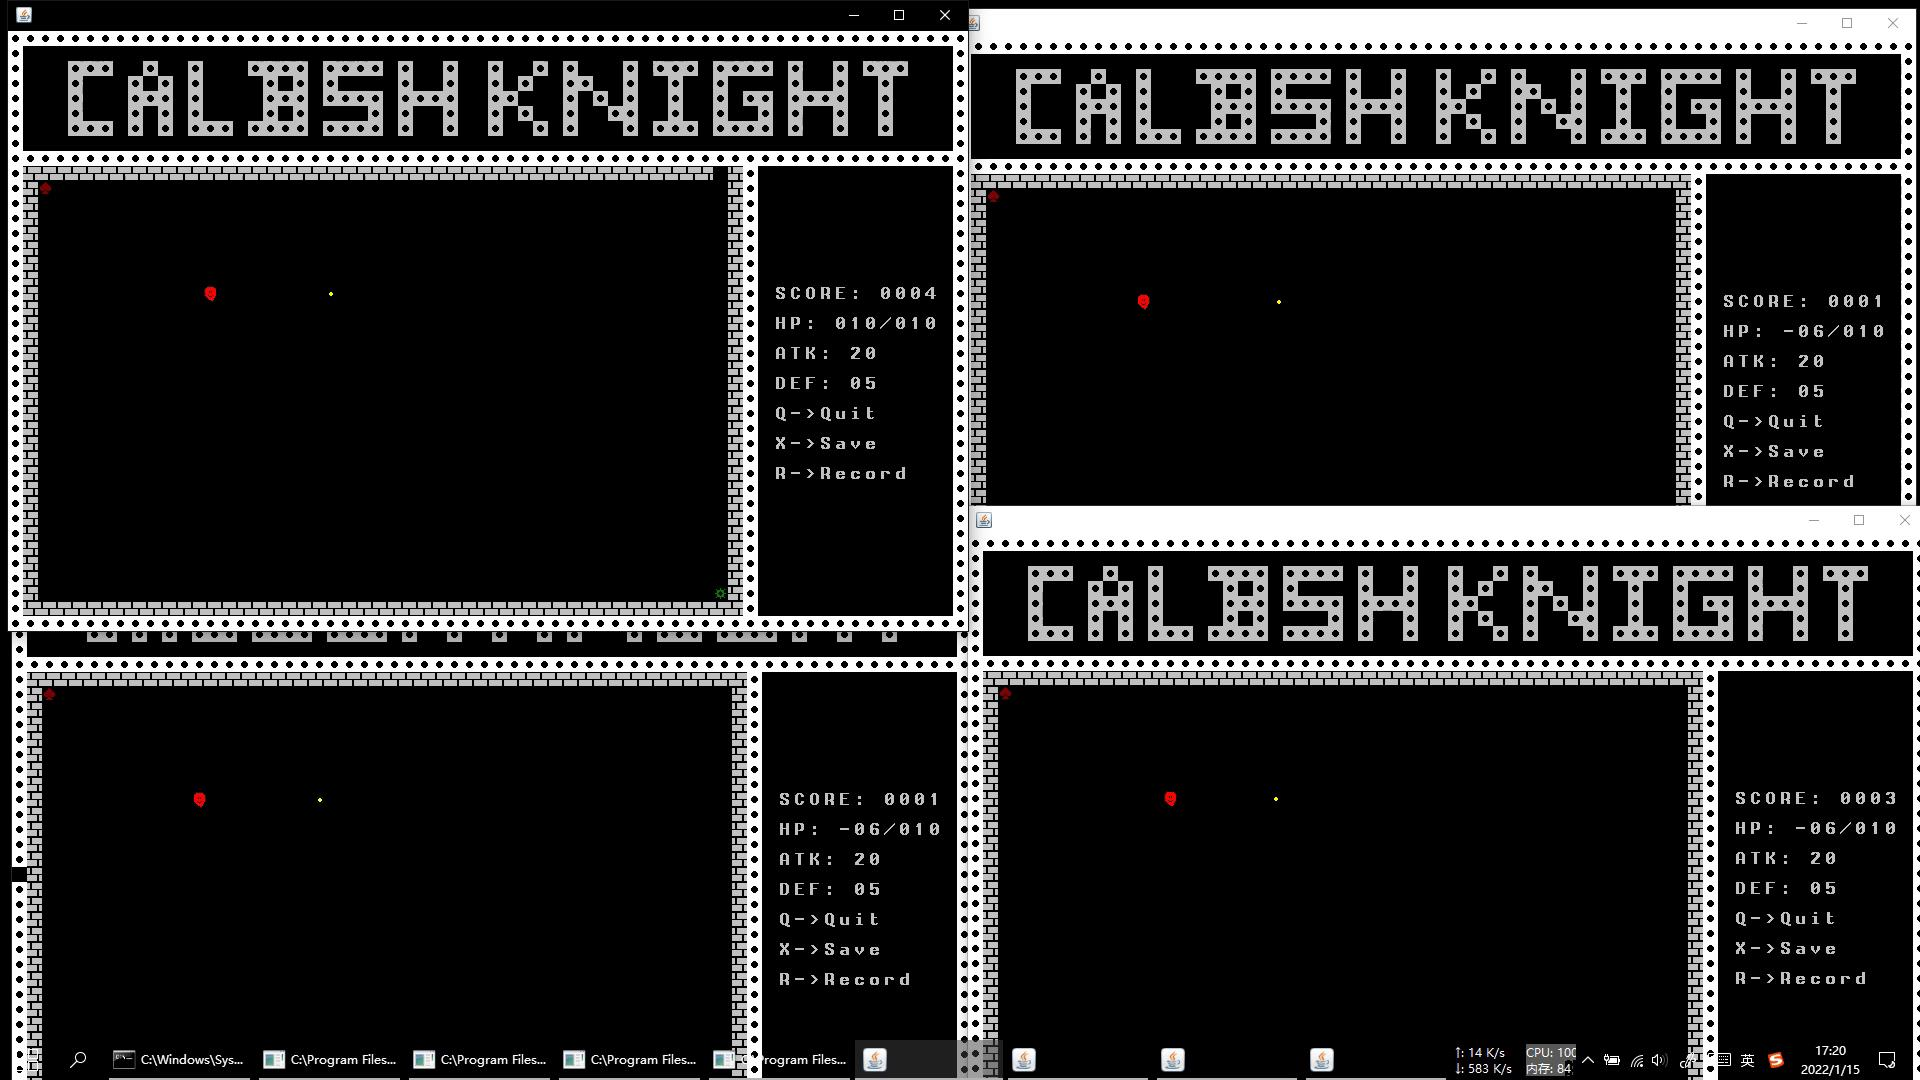
\includegraphics[width=0.30\textwidth]{ref/1-2-3-2.jpg}}
    \subfigure[胜利]{
    \label{Fig.s1233}
    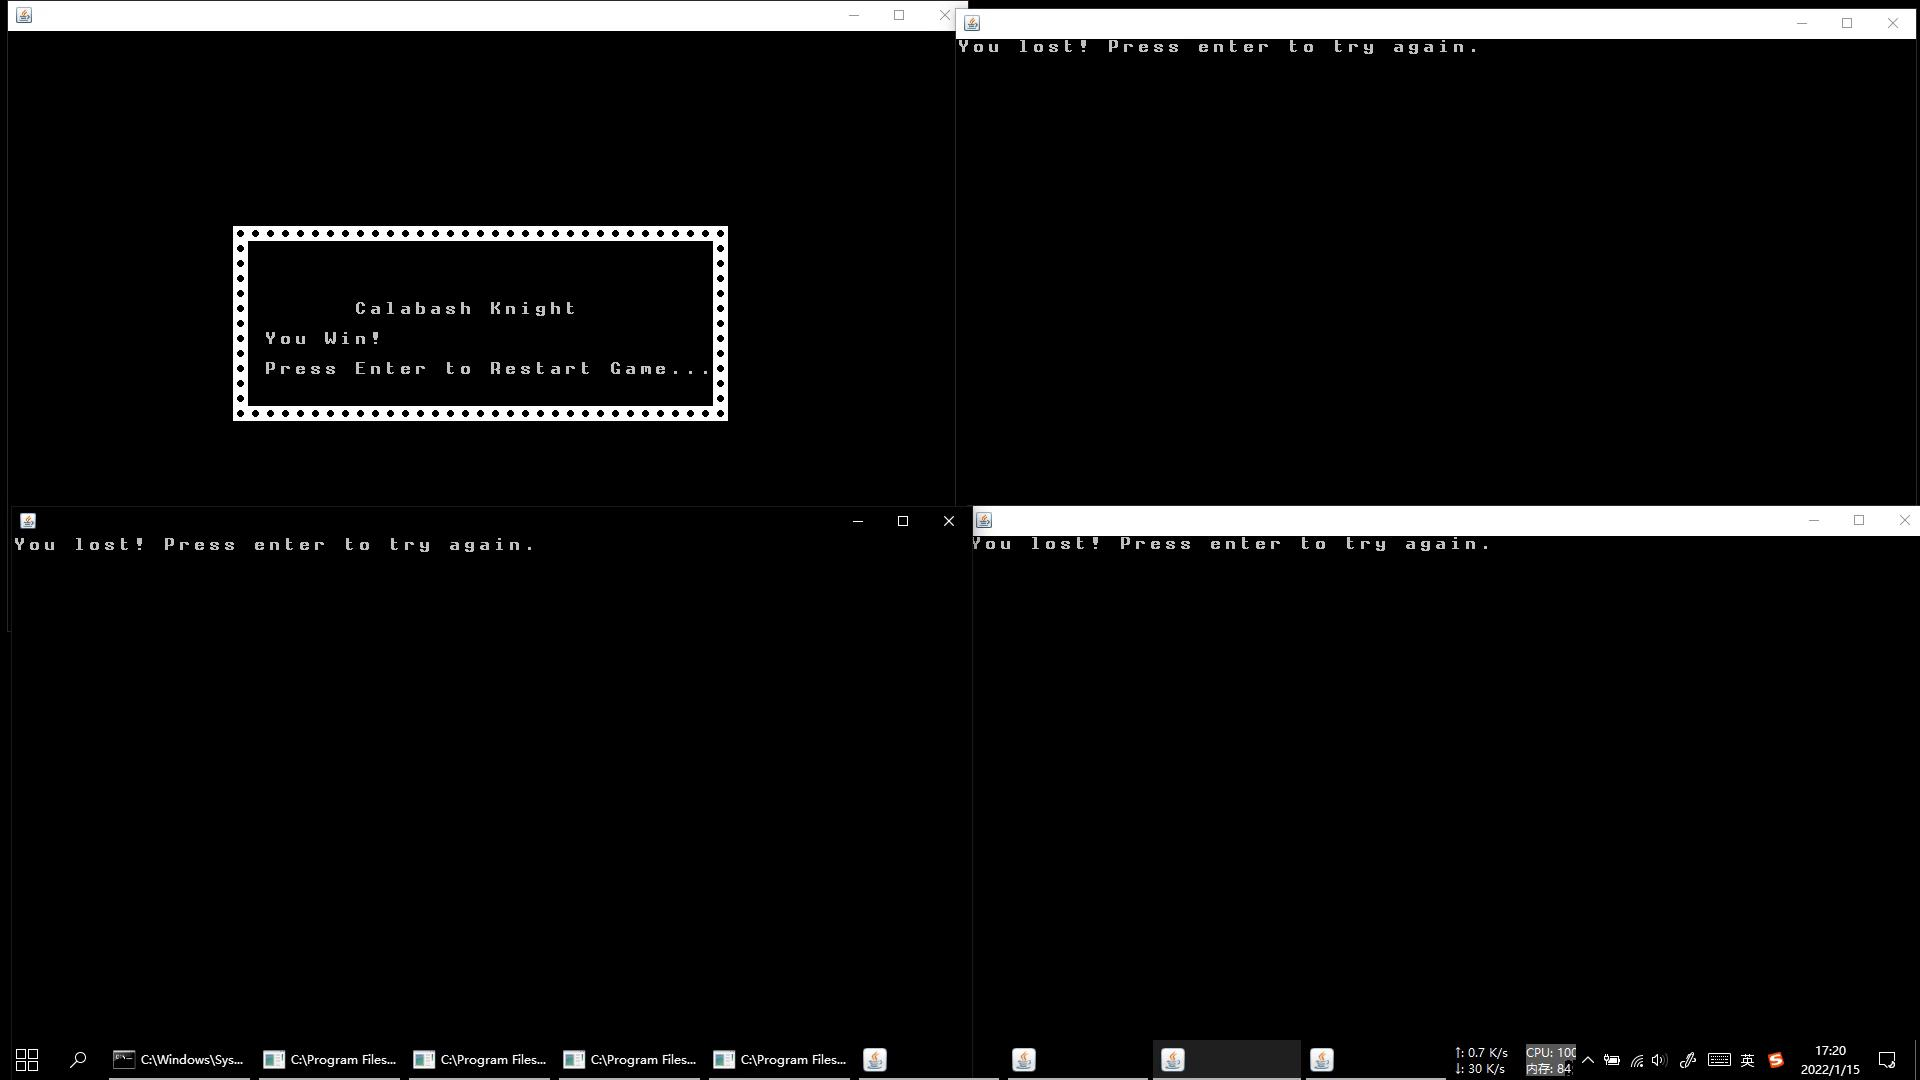
\includegraphics[width=0.30\textwidth]{ref/1-2-3-3.jpg}}
    \caption{3.0版本}
    \label{Fig.f123}
\end{figure}

启动方式(以四位玩家为例):

\begin{enumerate}
\item 服务端:

其中4表示玩家数量。

\lstset{language=bash,numbers=none}
\begin{lstlisting}
java -jar app.jar -s 4
\end{lstlisting}

\item 客户端

其中127.0.0.1为服务端IP地址,1表示该玩家的id,4表示玩家总数。

\begin{lstlisting}
java -jar app.jar 127.0.0.1 1 4
\end{lstlisting}

\item 为了方便调试,编写批量启动脚本

\lstset{language=bash,numbers=left}
\begin{lstlisting}
@echo off
echo client num is: %1
start java -jar jwork05-2.0-jar-with-dependencies.jar -s %1
set /a arg = %1
set /a num = %arg% - 1
for /l %%i in (1,1,%num%) do start java -jar jwork05-2.0-jar-with-dependencies.jar -c 127.0.0.1 %%i %1
\end{lstlisting}

\end{enumerate}

\section{设计理念}

\subsection{代码总体设计}

\subsubsection{类图}

\begin{figure}[H]
    \centering
    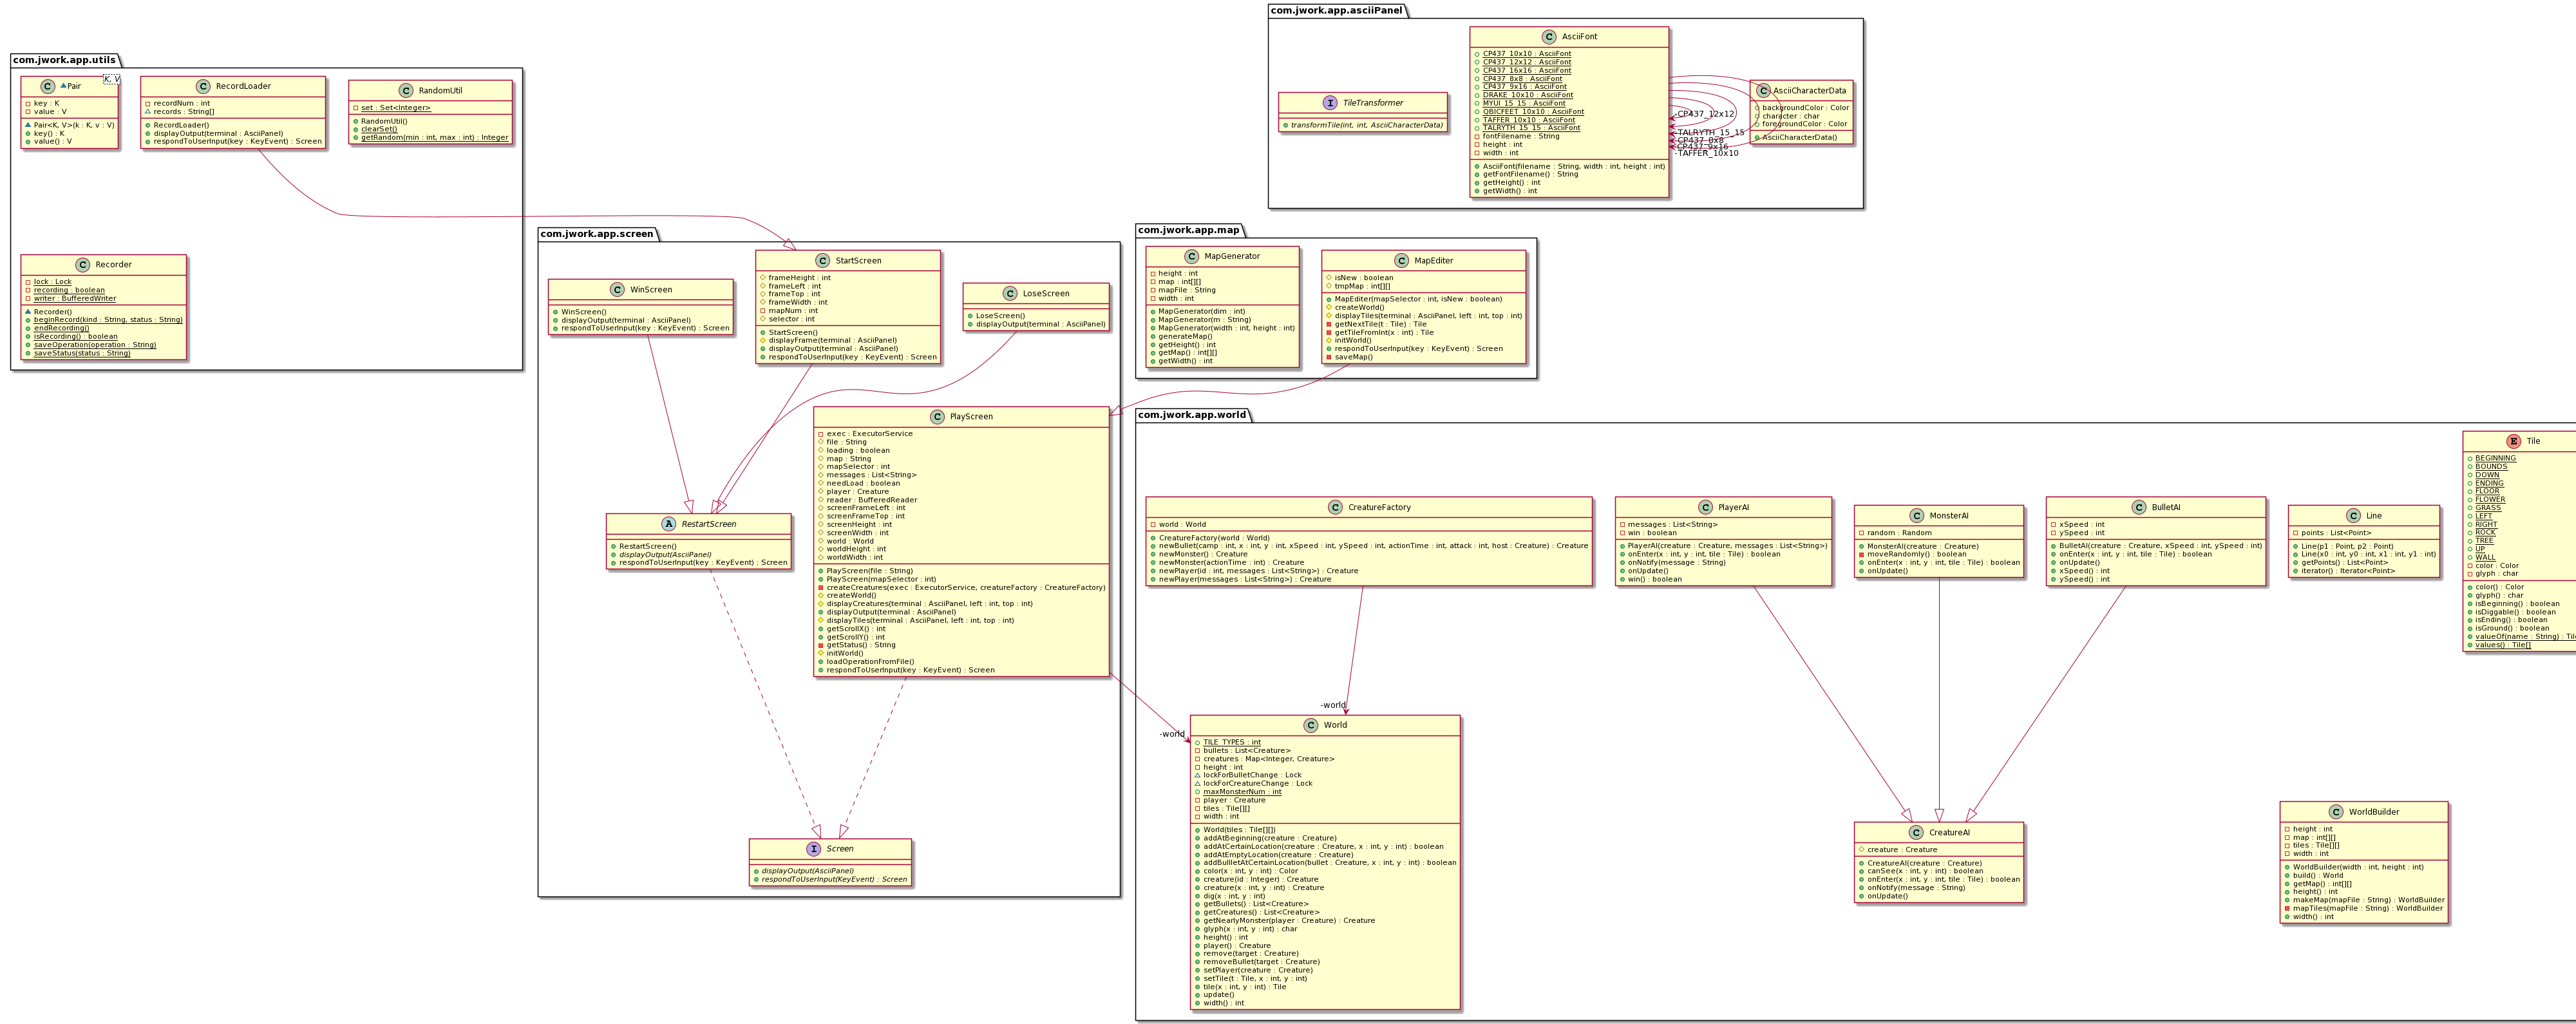
\includegraphics[width=1\textwidth]{ref/2-1-1-1.png}
    \caption{类图}
    \label{Fig.f2111}
\end{figure}

\href{https://plantuml.io/plantuml/png/lLdTRjlA4RxFKn3fpGgMZUEqFJqj0kFuXtA4AB8hoSSDWY1OYoEPDRaabYj7GfgyI9-YrmNwDaLVexjSxc0vIybs30H8O7BcczdP-PaThdwj59TgbMVH__xrx__-ypylIZw_uqk8vaL-yFVFXRmxu6Lvi59fLaLVNaJHjtd6gogwvAby_ROV_NPKKwDeFxg3JVINw6tpTi-p5UZtt-htRvu0kzDa_NHlkBsQlMU4MG_5zwoufbW5N_L_k-w4YwJ8hxGvk6u5IiEce5uFXO8bI6sItfLAvr-jCa-8kVNc6N2fPLYFWfUWB9xbgT2AKw7wKSxNzj5Or2o3Wcq3OLx8P5Jm12IQA6lYU9LR9TOb3RKonYkPYkM7ZyvUJmTQdAHLcV7DnKgLAyKKI6qUpxJmSJLFqqik87DG2LLPY6HMN5KWXyBWc-309hu7kulfN0A8q7RVxgoOcs2Dp1_ShRybRRNctnH51bnGo6UPQZCr_sIrM824vDeIMh1lk2hkz0QMgR1KTfUA11tKZupaga9243mGoSGP5eOshNmcsarX5R-7YnAafXM25Uw9h4e4fhLbhDD0J9AlMyfBFsH9z0K3SRBACb37Gmp4Ube299WzXhIXf3qKOpgqsWm9cdlQFFPRElejSUVuGiH2WMHh1Ba7bMP6sKp_yHo7ObTbmXLW0ErAhDSoRaE9c7Te8sxuTr773gmUVEtU9jOt5rE0O2VK-6ViULoeTB5XELIL2IX6lCifuLO7VAuAkS40rncWbLoRlrO5nR8MngqZuBCDEvlpl7IsqzrqHX_V-DpazopD0IbAwKHrRxT5fNmV-q51AzuLeZAEtCsbItMZBpE-qU0KBMoyN9bcb5RgjVNrqKxfnybWQ3H80CQZBFIwA7fftexi2ZMEbOUQLvFxKVdAFVTyoFedz3O-hG-HPfzGP0cgLb6nNkUgfdDoLLZ_3fiNX7ZRQ3pjDGzP7sTQp9vhZKB4TPUH5SsBUx1IsOOzltXsruQDcsVubWYwaaa5rOmgklQqFOj-N2km16qvSQPn0eXLNYyHVN7zF3uVZiV3yJazS4ukhiPdKqezkxWUKreyFkkG7umkBYOTnEiue9vFZgV1IgDuCAEqoV3yJKYyE7rBQRD975FQrIMbN1-FHdIWc1TP8Kr4pT-6jimsvQscpM-vjA8Mndeju9u56geFJQiJCsm8CX4WzonTBlbD1ftCM2JRvCvbiH89OU5SUx5WWkTUeZIvXVlrmHLpx0yVEqTEUnvWqio6e_ZJxFrbFBNPIvruKvyMM0EkEbnLkS8nW7UyT3DrFwB0MqYNjyeVQEjnSL18UnwTtdAnX6PwR0ESgX2oPoRjfZFXk4ntKDP5Jbl_Vbsb5VhgmqVi4ucwzKSHwp16uQuwUP8SAqoBRTqHaQSW5K-5teAT5pixp-uv17N5UQasg6dtoiRB6QZG01lWfooFDKDnj8QSHVPaRb8ZF8GH5oeCiKcwz67qKBJ9P8k092nY76atQWnSPXitY0H9H4t3ba6D8ot4rW4PTgtshbb8WZbJcU9IcqGZYtoxw-se2fGzwcYI4939RQQQ90_pm26LWGNCHgp1hEWPfgiATnsqevDLck6N9EqMbfJpqhvZhJwjX74Hvh7xhPNmYz80MG_dQym9tU4q6QtO5TAStu61QxC7QTPkthurkBlIRA9w79xuS-V7ebReVIfga-B438VuwPHMO_Zi5RYbghpKq62hA6xid486vbF3kP9ewldVPc2RgACrjnDsovsN4_qeWuN2YQee_H3jsm9TjnCMCn0XvcqWYtmebCjN13Mx5wb2qvvy6s8NglYz2JKPJpNb78GTl9-QrpG9jkQrlmXBqXoT579prDR9Vh0ebXPgTueqzIPC_ivIGSRrepEtgfti9U-eg62AHAFG8ptjvej-I5WT62TOmrnBnFhFIdjd2l8-dRkSMT3GQ5fMyFRjbgMRI59eK3cMlklpHNC5G7t55wmGZZUMhj-IrdNQf2OqNElRWUGvZB3EGjwiA3jODkOTZ3gsFZsug40QqO5qgcBF2mzhURuNyWFNzlmn5V3WPztnxHkSVuU2NaNA8veQhlB4nlRux7r-4yLgr8uhiknlf7wHyHuPs5ERcyiUJUkmavgQm8jHquPDJsFVV-lCRoebTHZm-hd-CO8q1AJkw0cUAwClJklNxxPBkmVaWiyX8hOyRzLmFL_CRs1JwWVJf4pvaY93Ub3o2onsIiHwz0yi_DPorH_siptVAbeYTM_fJjaV-Fl5TIf8m932Ve0PsuuzZfgzewzUJdy0c-23FEEAez4tMikola2elxteDvYJQN-6B0e9suN2rSXmKmC6XL1enUdb7tx_fq-7FwqFzUqbyid7EC9UhGzVFGBsy_hmvuTXlwn_UHZqvmTKdKsEtyOFs__k_TNmq-4VzRzTgB-U34y7SJnxMD_iU3289u_1ZIRlPsyUMde_McYQwREj6wFkwRDxf4JDR47LzAD7J8bgu5b0ZucT8oEP34blDSVSJ79HwTJDGMBYAKSp06OCizQ5EKpQhgb0R_JRtp-AefVxzH3oifbNoE7VYK5_EQwNuYyZv8QuLaXt8Z7DTwCmptV2_8ppWVXffu7_EFAcgXVUs6rOxIFMT-71WUOsP0G5d2dIE_LX3-vY-ZzrM_xKu-Ble8RZ_VBt0d-ye9pQ-ax6ho2ILPxz7m00}{查看原图}

\subsubsection{关键类介绍}

\begin{enumerate}
    \item App
    App主类,用于监听键盘事件及处理各个Screen的切换。
    \item Flasher
    用于定时刷新屏幕,可以设定FPS。
    \item World
    实体的载体世界,所有的游戏实体都在world中管理。
    \item WorldBuilder
    用于创建世界,传入世界的宽度和高度,可以创建不同种类的世界,本项目中可以根据
    MapGenerator类的创建结果来创建世界地图。
    \item MapGenerator
    生成世界地图,可以读取文件中的内容来生成地图。
    \item MapEditer
    地图编辑器,由于主要的内容与PlayScreen相似,所以继承于PlayScreen。
    \item Creature
    游戏中生物的基类,包含所有生物共有的属性和方法,如移动、攻击等,是一个单独的线程。
    \item CreatureAI
    操作Creature的“大脑”,用于进行一些判定,如canSee, canEnter等。
    \item Player/PlayerAI
    继承于Creature的玩家,可以由用户操作。
    \item Monster/MonsterAI
    地图上随机游走,并攻击可见玩家的怪物。
    \item Bullet/BulletAI
    玩家或怪物发射的子弹,统一有BulletManager管理。
    \item BulletManager
    用于统一管理子弹,每一个生物实体拥有一个BulletManager类,该类为一个单独的线程。
    \item CreatureFactory
    用于游戏世界初始化时创建生物,可以在随机位置/起始位置/指定位置生成玩家/怪物。
    \item Recorder
    用于记录游戏状态/操作,将记录内容保存成文件。
    \item RecordLoader
    用于加载记录内容文件。
    \item EventManager
    玩家操作管理者,将键盘事件整理为一个个的操作并存入缓存,由玩家AI读取。在3.0版本
    中,该类也用于网络通信,将本地的操作缓冲发到服务器上,并接收服务器传来的其他玩家
    的操作。
    \item Screen
    屏幕基类,用于显示屏幕内容。
    \item RestartScreen
    继承于Screen类,可以处理键盘操作,是其他屏幕类的父类。
    \item StartScreen
    开始屏幕,用于选择/编辑地图或加载记录。
    \item PlayScreen
    进行游戏是显示地图和实体。
    \item WinScreen/LoseScreen
    游戏结束时显示界面。
\end{enumerate}

\subsection{设计思路}

整体的设计思路是基于面向对象的,将所有的实体都定义为一个类,实体间的交互通过类的方法
来进行通信,类之间如果有属于关系则使用继承的方法,如玩家属于生物,则Player继承Creature。

每一个生物都独立开创一个线程来提高生物处理事务的性能。在涉及到所有生物共用的信息,即
临界区时则需要用线程锁来控制,例如读取当前世界中的生物时,由于不同的生物操作可能导致
当前世界的生物发生变化,所以需要加锁来进行控制。

网络通信的部分使用NIO Selector进行管理。服务端接收客户端的请求后将其注册到Selector
中,通过selector的判断来对客户端的读写进行管理。

\subsection{优缺点}

\begin{enumerate}
    \item 优点
    \begin{enumerate}
        \item 使用面向对象的方法,更加模块化,减少代码之间的耦合度,提高代码
        复用性,也可以缩短开发周期。
        \item 使用多线程的方式,相比于单线程,可以更大程度的利用CPU资源,提高
        程序运行效率,在代码开发过程中也可以忽略线程之间的先后关系,降低代码复
        杂度。
        \item 使用NIO的方式,与阻塞式的IO相比,可以在单个线程中处理多个服务端
        的请求,避免过多的线程等待读写造成资源的浪费。
    \end{enumerate}
    
    \item 缺点
    \begin{enumerate}
        \item 面向对象的方法中,类之间的继承关系如果处理不当,就会使代码的维护
        变得很困难,代码可读性下降。
        \item 多线程共享的变量、数据等可能会造成数据的错误,如读取脏数据等,此时
        就需要通过加锁来控制,但过多的锁又会导致效率低下。
    \end{enumerate}
\end{enumerate}

\section{技术问题}

\subsection{并发控制}

在多线程编程时并发控制尤为重要,本项目中,主要的并发控制在于各个线程共享的变量
的处理,如多个生物体同时进入同一个地面、多个子弹同时击中同一个生物等等。

要处理这些问题,最好的方式是加锁控制。因此,我在world中地块内容修改时加锁,这样
就可以避免两个生物同时进入一个地块;在子弹对生物体进行实质的攻击(造成伤害)时
加锁,这样就可以让同时达到的子弹实际上有先后顺序,避免错误。

\subsection{通信控制}

主要采用NIO的Selector的方式。数据同步的逻辑为,在服务端和客户端都维护两个队列,
一个事件缓存队列,一个事件执行队列,当用户按键时,将玩家ID与事件存入缓存队列。
在客户端中,定时将缓存队列的内容发到服务端,服务端接收后存入服务端的缓存队列中。
在服务端中定时将缓存队列的内容加入执行队列,并发给所有客户端,客户端接收后存入执
行队列。如此便可以保证所有的客户端和服务端所执行的事件都是相同的。


\begin{figure}[H]
    \centering
    \subfigure[NIO Selector]{
    \label{Fig.s3211}
    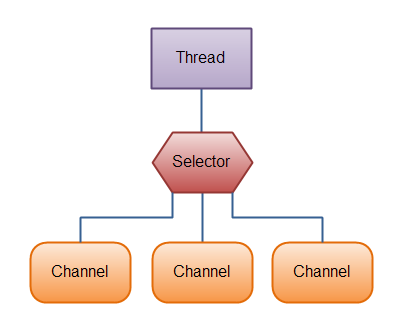
\includegraphics[width=0.45\textwidth]{ref/3-2-1-1.png}}
    \subfigure[事件队列]{
    \label{Fig.s3212}
    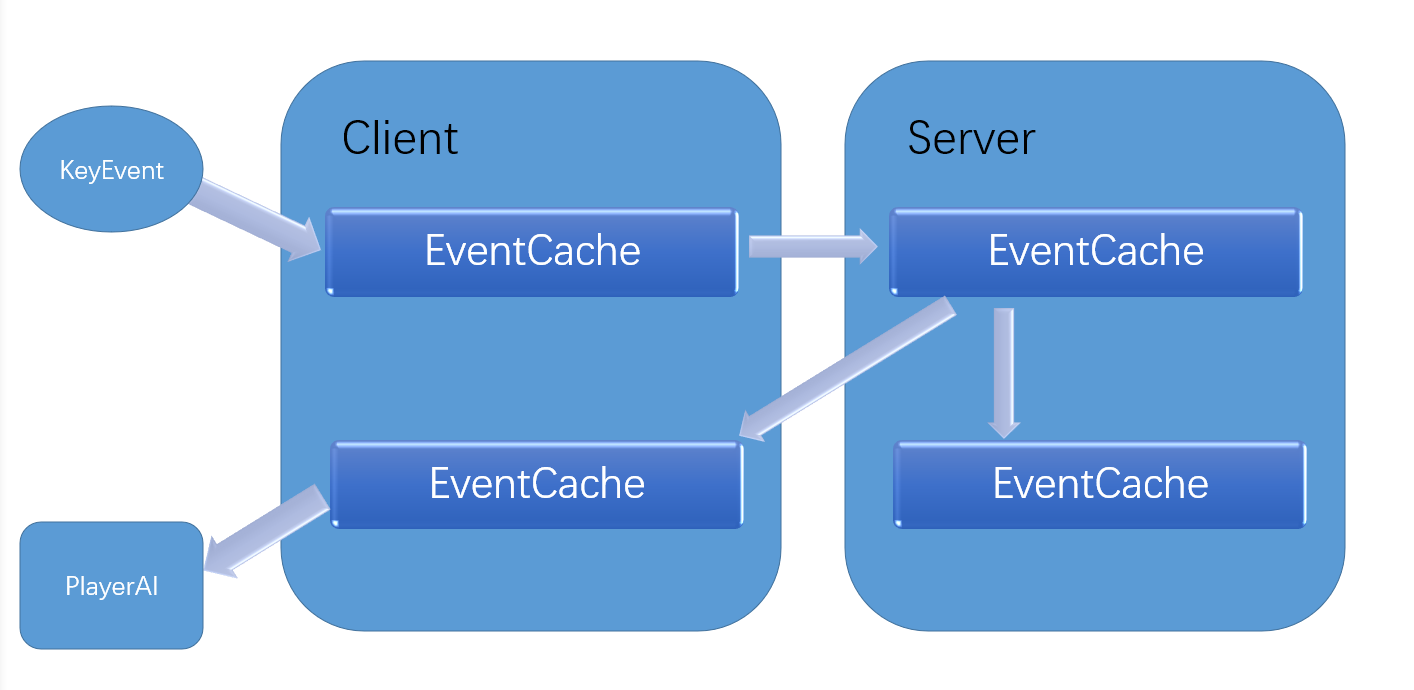
\includegraphics[width=0.45\textwidth]{ref/3-2-1-2.png}}
    \caption{通信控制}
    \label{Fig.f321}
\end{figure}

\subsection{界面显示}

通过一个单独的线程Flasher来定时刷新屏幕内容,实现相对稳定的刷新率。
屏幕显示的内容主要通过ASCIIPanel来实现,并通过修改贴图的部分内容
来实现多样化的UI设计。

\subsection{文件存取}

本项目中,地图的保存、加载,记录的保存、加载都需要进行文件操作,但
默认地图是在资源文件中,最终是要打包到jar文件中的,是不可编辑的,
我在开始编程时,由于项目本身的资源文件可以编辑,所以我将所有的文件
都存在了资源文件夹中,最终导致打包的jar无法正确运行,我的解决办法就是
在游戏初始化时将两个默认地图的文件拷贝到运行目录中,并将新增的地图和
记录的游戏状态和操作都存在运行目录中,以实现文件的读写。

\section{工程问题}

\subsection{包管理}

从jw05阶段开始就是用maven进行包管理,通过在pom.xml中包含所需的各种
依赖和插件等,可以减少代码开发以外的额外精力消耗。

\subsection{插件管理}

同样使用maven进行插件管理,这里我用到的插件有:

\begin{enumerate}
    \item 依赖打包插件(maven-assembly-plugin)
    用于将依赖打包进jar文件,否则jar文件无法运行.
    \item 测试覆盖度报告生成插件(jacoco-maven-plugin)
    用于自动生成单元测试覆盖度。
    \item UML类图生成插件(urm-maven-plugin)
    用于自动生成UML格式的类图。
\end{enumerate}

\subsection{自动化测试}

使用maven进行项目管理时,在test文件下对应目录编写测试文件并添加@test,就
可以在项目的life cycle中自动运行测试用例。

\subsection{自动生成UML类图}

由于项目较为复杂,手动编写类图复杂而且繁琐,又容易出错,因此使用自动构建
类图的插件就可以大幅度降低工作量。在这里我使用开源项目\href{https://github.com/iluwatar/uml-reverse-mapper}
{uml-reverse-mapper}来实现自动生成类图,具体使用方法:

将仓库克隆到本地并编译其中的urm-core项目,将生成的urm-core.jar与自己的项目
jar文件放入同一个文件夹,执行以下命令即可:

\lstset{language=bash,numbers=none}
\begin{lstlisting}
java -cp jwork05-3.0-jar-with-dependencies.jar;urm-core.jar com.iluwatar.urm.DomainMapperCli -p com.jwork.app
\end{lstlisting}

其中jwork05-3.0-jar-with-dependencies.jar是我的项目生成的jar文件,com.jwork.app是
所要生成类图的包名。

\section{课程感言}

一直以来我都希望在大学期间能够有更多的项目实践经历,这门课程的整体思路就是以
一个JAVA项目为主体来展开的,我很高兴也很喜欢选修这门课,课程项目的实践让我
对面向对象的设计理念有了更深入的认识,网络通信、并发控制等内容也让拓宽了我的
知识面,第一次尝试使用工程管理工具如maven等进行项目管理,体会到了有效的工程
方法对开发效率的提升。

对于这门课的授课形式,老师讲课以启发为主,主要要求我们自行探索,阅读相关书籍
和文档,可以在有限的课程时间内让我们掌握更多的知识,我认为比传统的灌输知识要
好得多。对于课程内容,我认为当前已经十分完善。

最后想说的一点就是拖延症要不得!即使一个时间很充裕的作业也可能因为拖延症而
晚交。。。

\end{document}
